% ============================================================
%  Domain model - PrepMeUp (SW4PRJ4, gruppe 3)
%  Kompilerer selvstaendigt:  pdflatex domain-model.tex
%  Bruges i rapporten med:    \input{assets/tikz/domain-model-body.tex}
%  (klip alt mellem \begin{tikzpicture} og \end{tikzpicture} ud,
%   eller \includegraphics den PDF, denne fil producerer.)
%  Notation: Larman kap. 9 - konceptuelle klasser, attributter uden typer,
%  navngivne associationer med multiplicitet. Ingen metoder, ingen teknologi.
% ============================================================
\documentclass[tikz,border=8pt]{standalone}
\usepackage[T1]{fontenc}
\usepackage[utf8]{inputenc}
\usepackage{lmodern}
\usetikzlibrary{shapes.multipart,positioning,calc}

\definecolor{deep}{HTML}{173330}
\definecolor{signal}{HTML}{C99700}
\definecolor{signalbg}{HTML}{FBF5E3}

\tikzset{
  % En konceptuel klasse: navn oeverst, attributter nedenunder (ingen metode-rum)
  cls/.style={
    draw=deep, line width=.6pt, fill=white,
    rectangle split, rectangle split parts=2,
    rectangle split part align={center,left},
    text width=34mm, inner sep=4pt, font=\small,
    align=left,
  },
  % Kun-navn-klasse (Package har ingen attributter)
  clsn/.style={draw=deep, line width=.6pt, fill=white,
    text width=34mm, inner sep=4pt, minimum height=10mm,
    font=\small\bfseries, align=center},
  assoc/.style={draw=deep, line width=.6pt},
  lbl/.style={font=\scriptsize, fill=white, inner sep=1.5pt},
  mult/.style={font=\scriptsize\itshape, inner sep=1.5pt},
}

% \cls{node-navn}{position}{Klassenavn}{attributter adskilt med \\}
\newcommand{\cls}[4]{%
  \node[cls] (#1) at (#2) {\textbf{#3}\nodepart{two}#4};}

\begin{document}
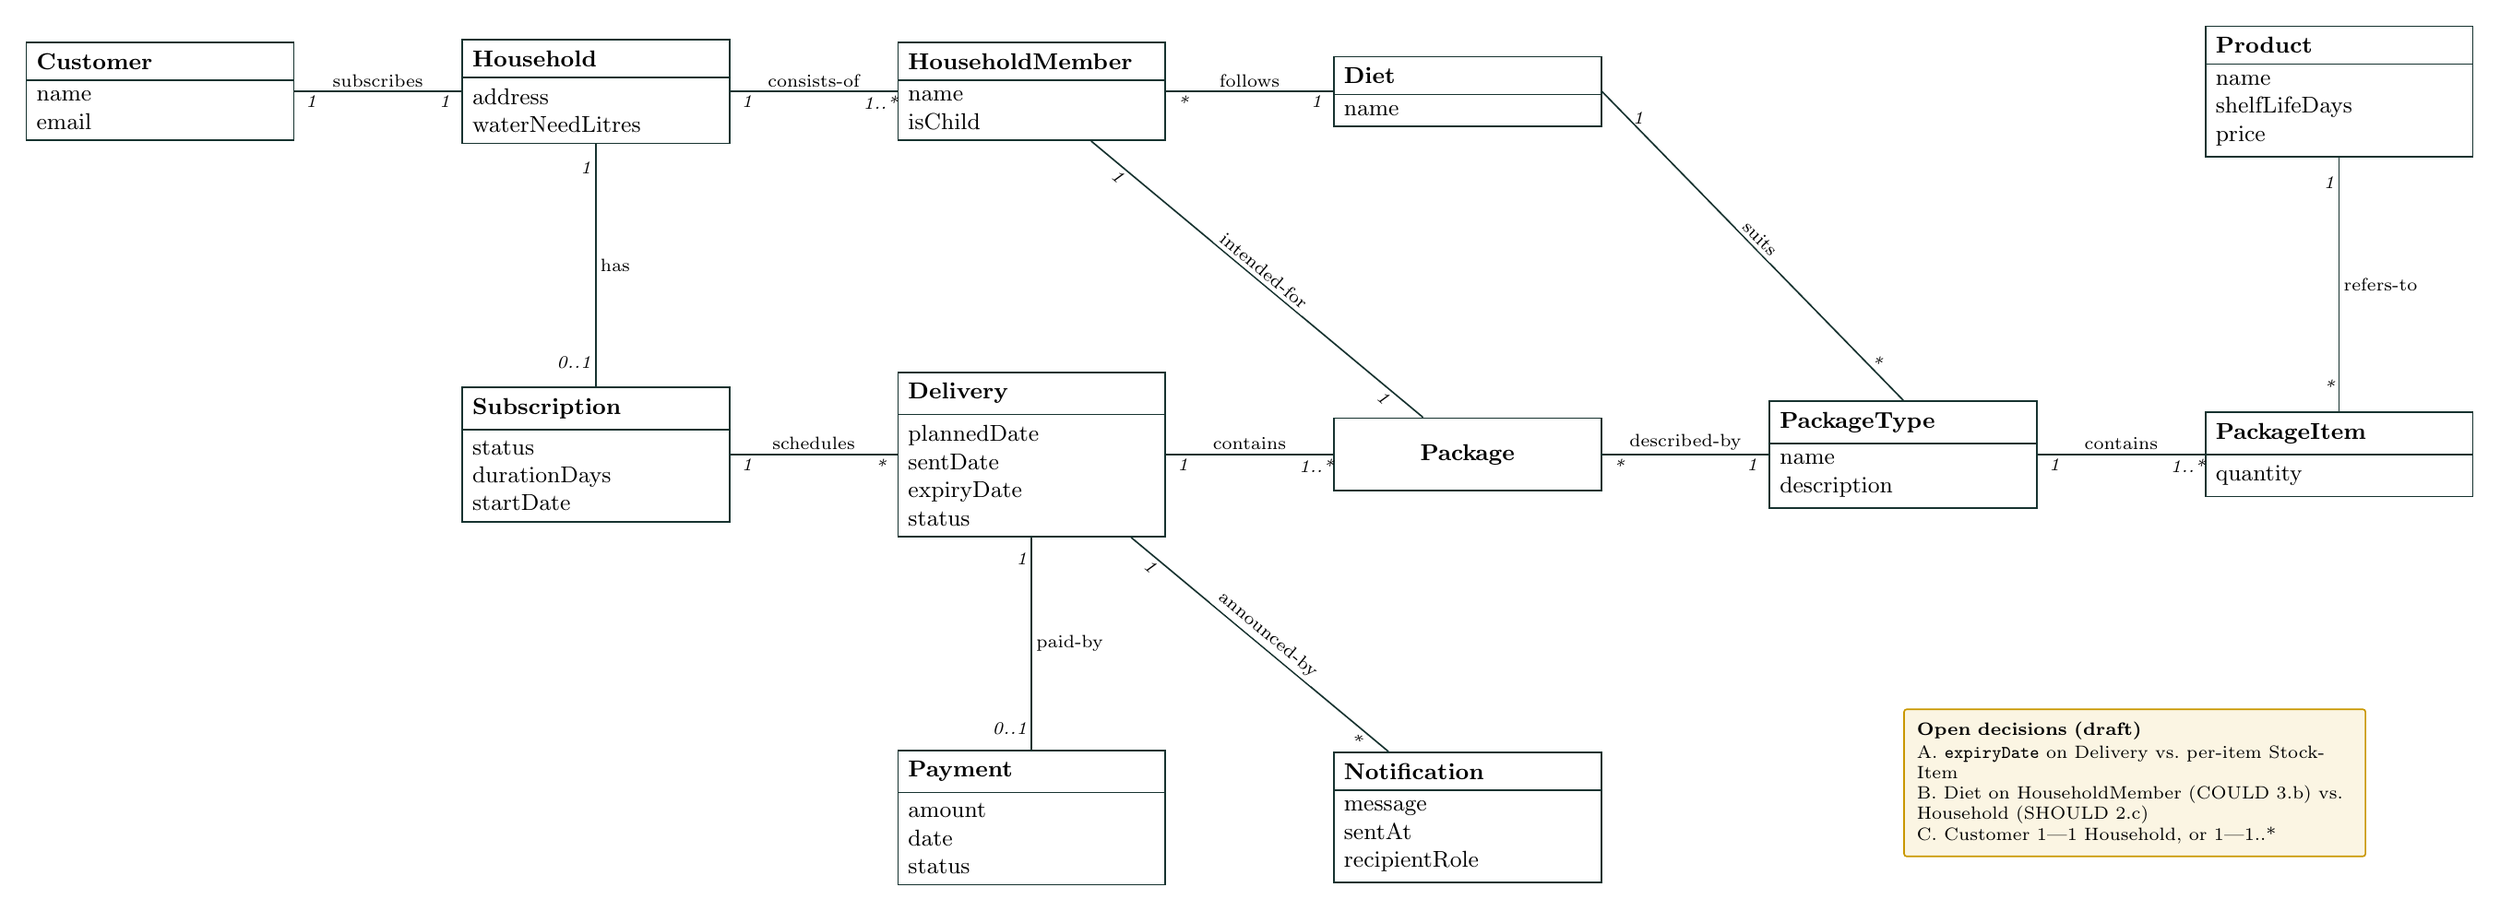
\begin{tikzpicture}[x=1mm,y=1mm]

% ----- raekke 1 -----
\cls{customer}{0,0}{Customer}{name\\email}
\cls{household}{60,0}{Household}{address\\waterNeedLitres}
\cls{member}{120,0}{HouseholdMember}{name\\isChild}
\cls{diet}{180,0}{Diet}{name}
\cls{product}{300,0}{Product}{name\\shelfLifeDays\\price}

% ----- raekke 2 -----
\cls{subscription}{60,-50}{Subscription}{status\\durationDays\\startDate}
\cls{delivery}{120,-50}{Delivery}{plannedDate\\sentDate\\expiryDate\\status}
\node[clsn] (package) at (180,-50) {Package};
\cls{packagetype}{240,-50}{PackageType}{name\\description}
\cls{packageitem}{300,-50}{PackageItem}{quantity}

% ----- raekke 3 -----
\cls{payment}{120,-100}{Payment}{amount\\date\\status}
\cls{notification}{180,-100}{Notification}{message\\sentAt\\recipientRole}

% ----- associationer (navn i midten, multiplicitet ved hver ende) -----
% Hjaelper: \assoc{fra}{til}{navn}{mult ved fra}{mult ved til}{navn-side}{mult-side}
% Navn og multipliciteter saettes paa hver sin side af stregen, saa de ikke kolliderer.
\newcommand{\assoc}[7]{%
  \draw[assoc] (#1) -- node[lbl,#6]{#3}
    node[mult,pos=.1,#7]{#4} node[mult,pos=.9,#7]{#5} (#2);}

\assoc{customer}{household}{subscribes}{1}{1}{above}{below}
\assoc{household}{member}{consists-of}{1}{1..*}{above}{below}
\assoc{member}{diet}{follows}{*}{1}{above}{below}
\assoc{household}{subscription}{has}{1}{0..1}{right}{left}
\assoc{subscription}{delivery}{schedules}{1}{*}{above}{below}
\assoc{delivery}{package}{contains}{1}{1..*}{above}{below}
\assoc{package}{packagetype}{described-by}{*}{1}{above}{below}
\assoc{package}{member}{intended-for}{1}{1}{sloped,above}{sloped,below}
\assoc{packagetype}{packageitem}{contains}{1}{1..*}{above}{below}
\assoc{packageitem}{product}{refers-to}{*}{1}{right}{left}
\assoc{delivery}{payment}{paid-by}{1}{0..1}{right}{left}
\assoc{delivery}{notification}{announced-by}{1}{*}{sloped,above}{sloped,below}

% PackageType -> Diet: skraa kant, saa den ikke krydser Package
\draw[assoc] (packagetype.north) -- node[lbl,sloped,above]{suits}
  node[mult,pos=.12,right]{*} node[mult,pos=.88,above]{1} (diet.east);

% ----- note med aabne beslutninger (slettes foer rapporten) -----
\node[draw=signal, fill=signalbg, rounded corners=1pt, line width=.6pt,
      text width=60mm, inner sep=5pt, font=\scriptsize, align=left,
      anchor=north west] at (240,-85) {%
  \textbf{Open decisions (draft)}\\[1pt]
  A. \texttt{expiryDate} on Delivery vs.\ per-item StockItem\\
  B. Diet on HouseholdMember (COULD 3.b) vs.\ Household (SHOULD 2.c)\\
  C. Customer 1---1 Household, or 1---1..*};

\end{tikzpicture}
\end{document}